\documentclass[a4paper,11pt]{article}
\author{ 杨旭鹏  \  PB17000234}
\date{2019年秋季}
\title{计算物理A 第十四题}

\usepackage{ctex}
\usepackage{amsmath}
\usepackage{amsfonts}
\usepackage{graphicx}
\usepackage{lastpage}
\usepackage{hyperref}
\usepackage{appendix}
\usepackage{geometry}
\geometry{left=2.5cm,right=2.5cm,top=2.5cm,bottom=2.5cm}
\makeatletter\def\@captype{table}\makeatother
 


\begin{document}
\maketitle

\section{题目描述}
推导三角格子点阵上座逾渗的重整化群变换表达式 $p'= R(p)$,其中端-端连接的条件是3个格点中的2个是占据态,求临界点 $p_{c}$ 与临界指数$\nu$,与正确值(表1.6.1.3-1) 相比较。


\section{推导过程}
根据计算物理讲义上的说明,有三角格子重整化的示意:
\begin{figure}[!htbp]
\centering
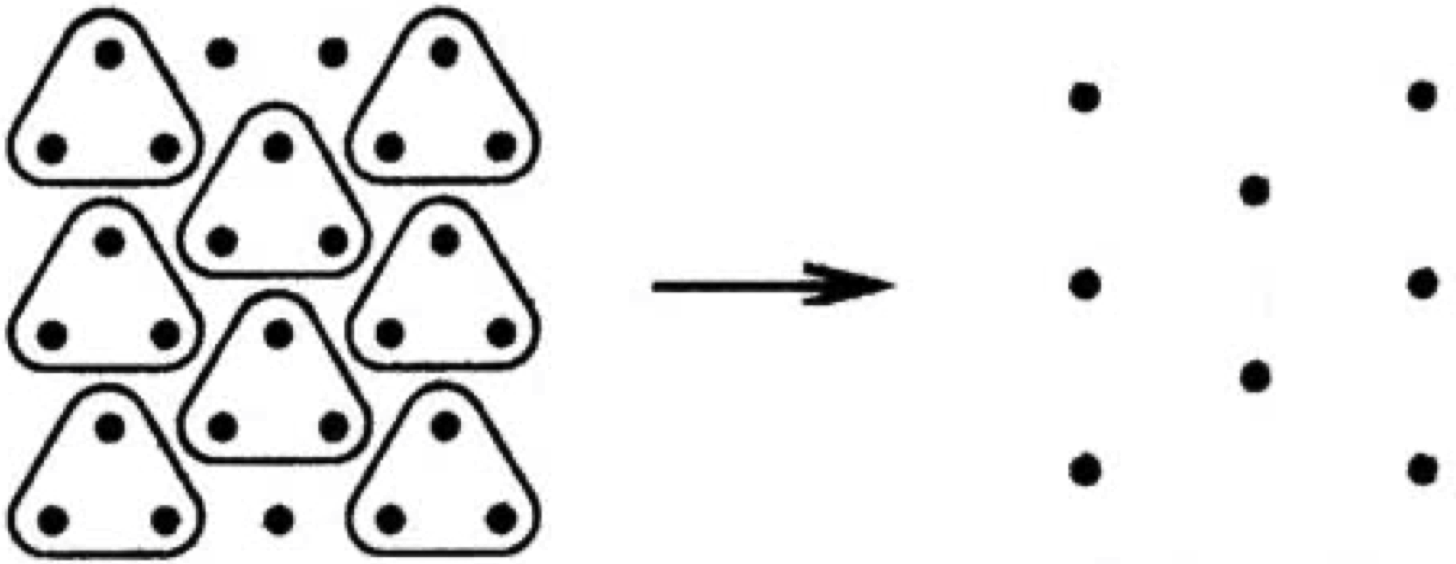
\includegraphics[width = 8cm]{lattice.png}
\caption{三角格子的重整化示意}
\end{figure}

可知放大因子$b=\sqrt{3}$。


根据题目给定规则,当占据态为以下4种情况时,认为端-端链接:
\begin{figure}[!htbp]
\centering
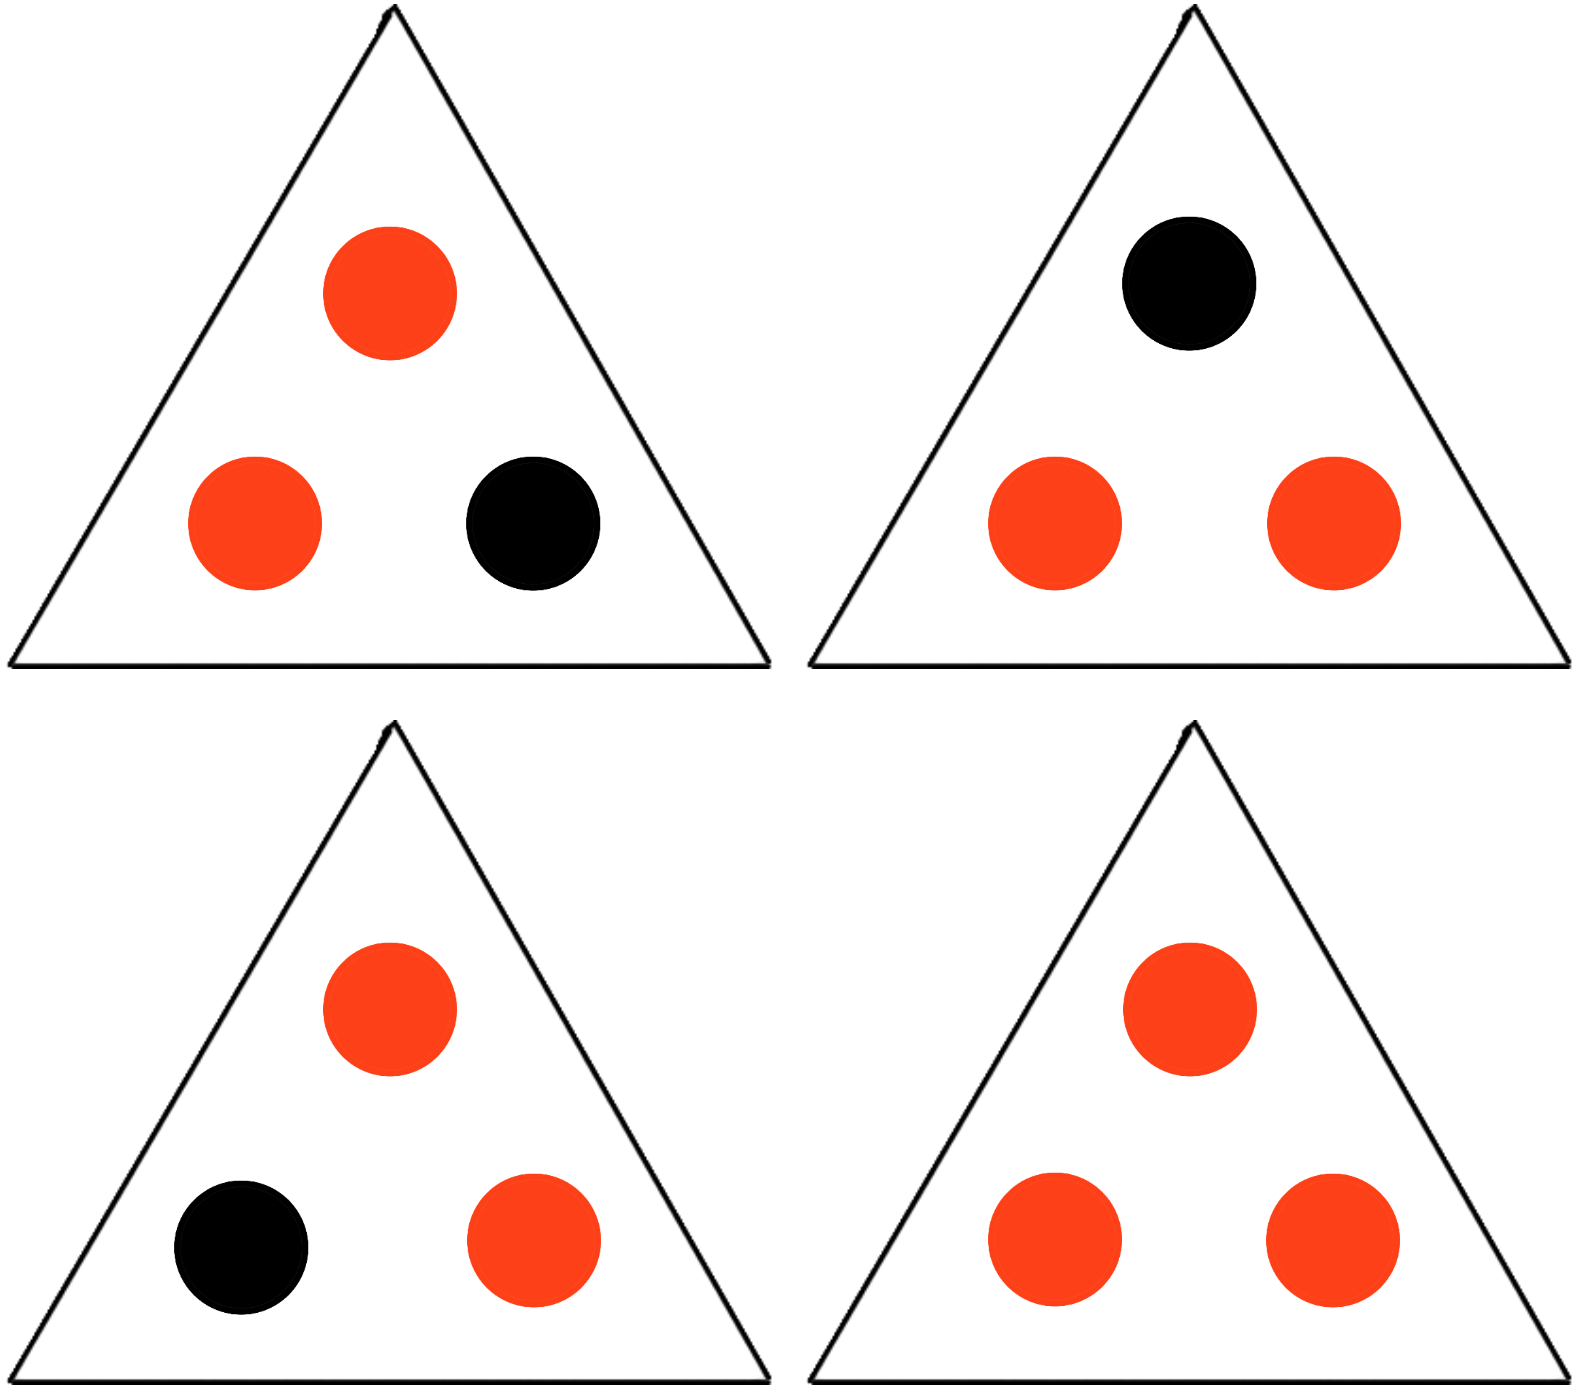
\includegraphics[width = 5cm]{occupy.png}
\caption{三角格子的重整化示意}
\end{figure}

其中红色代表占据态,黑色代表未占据态。我们容易写出变换表达式:
\begin{equation}
	p' = p^{3}+3p^{2}(1-p) = p^{2}(3-2p)
\end{equation}
\newline 当$p'= p$时$p'$为临界点$p^{*}$。有:
\begin{equation}
	p^{*} = (p^{*})^{2}(3-2p^{*})
\end{equation}

解得:
\begin{equation}
	p^{*} = \frac{1}{2}
\end{equation}
其中方程的解舍掉了对应稳定不动点$p^{*} =0$和$p^{*} =1$的情况。

即临界指数$p_{c} = \frac{1}{2}$

标度指数$\nu$利用公式:
\begin{equation}
\begin{aligned}
	\nu = \frac{lnb}{ln\lambda} &= \frac{lnb}{ln(\frac{dp'}{dp})_{p' = p^{*}}} = \frac{ln\sqrt{3}}{ln(6p'(1-p'))_{p' = p^{*}}} \\
	&= \frac{ln3}{2(ln3-ln2)} \approx 1.3548	
\end{aligned}
\end{equation}

与(表1.6.1.3-1)相比,对于三角格子点阵情况,有:
\begin{description}
\centering
	\item $p_{c} = 0.500000$
	\item $\nu = \frac{4}{3} \approx 1.3333$
\end{description}

两者比较,$p_{c}$完全符合,但$\nu$和理论值相比较还是有一定差别,但并不是很大,误差$|\varepsilon| \sim 10^{-2} $




\end{document}